\chapter{The Limits of Knowledge}
\label{les:7}

\begin{chapquote}{Lewis Carroll, \textit{Alice in Wonderland}}
``Down, down, down. Would the fall never come to an end?''
\end{chapquote}

Getting into Bitcoin is a humbling experience. I thought that I knew
things. I thought that I was educated. I thought that I knew my computer
science, at the very least. I studied it for years, so I have to know
everything about digital signatures, hashes, encryption, operational
security, and networks, right?

\paragraph{}
Wrong.

\paragraph{}
Learning all the fundamentals which make Bitcoin work is hard.
Understanding all of them deeply is borderline impossible.

\begin{samepage}\begin{quotation}
``No one has found the bottom of the Bitcoin rabbit hole.''
\flushright -- Jameson Lopp\footnote{Jameson Lopp, tweet from Nov 11, 2018 \cite{lopp-tweet}}
\end{quotation}\end{samepage}

\begin{figure}
  \centering
  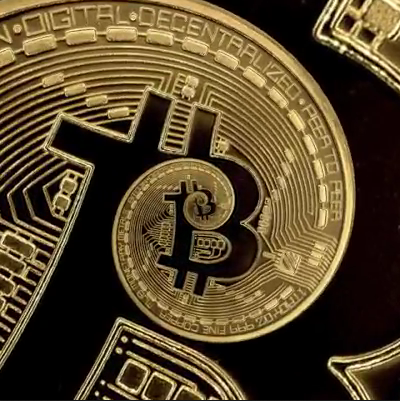
\includegraphics[width=7cm]{assets/images/rabbit-hole-bottomless.png}
  \caption{The Bitcoin rabbit hole is bottomless.}
  \label{fig:rabbit-hole-bottomless}
\end{figure}

My list of books to read keeps expanding way quicker than I could
possibly read them. The list of papers and articles to read is virtually
endless. There are more podcasts on all of these topics than I could
ever listen to. It truly is humbling. Further, Bitcoin is evolving and
it's almost impossible to stay up-to-date with the accelerating rate of
innovation. The dust of the first layer hasn't even settled yet, and
people have already built the second layer and are working on the third.

\paragraph{Bitcoin taught me that I know very little about almost anything. It
taught me that this rabbit hole is bottomless.}

% ---
%
% #### Down the Rabbit Hole
%
% - [Bitcoin Literature] by the Satoshi Nakamoto Institute
% - [Bitcoin Information & Resources][lopp-resources] by Jameson Lopp
% - [Educational Resources][bitcoin-only] by Bitcoin Only
%
% <!-- Twitter -->
% [Jameson Lopp]: https://twitter.com/lopp/status/1061415918616698881
%
% <!-- Down the Rabbit Hole -->
% [lopp-resources]: https://www.lopp.net/bitcoin-information.html
% [bitcoin-only]: https://bitcoin-only.com/#learning
% [Bitcoin Literature]: https://nakamotoinstitute.org/literature/
%
% <!-- Wikipedia -->
% [alice]: https://en.wikipedia.org/wiki/Alice%27s_Adventures_in_Wonderland
% [carroll]: https://en.wikipedia.org/wiki/Lewis_Carroll
